\begin{figure*}

\begin{subfigure}{0.5\linewidth}
\begin{minipage}{0.1\linewidth}
~
\end{minipage}%
\begin{minipage}{0.3\linewidth}
\centering
\textit{Early}
\end{minipage}%
\begin{minipage}{0.3\linewidth}
\centering
\textit{Late}
\end{minipage}%
\begin{minipage}{0.3\linewidth}
\centering
\textit{All}
\end{minipage}


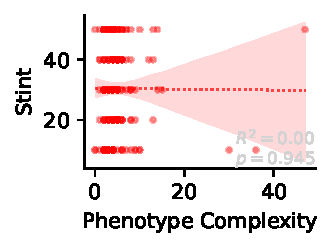
\includegraphics[width=0.39\linewidth,trim={0 1.2cm 0 0},clip]{binder-2025-12-10-complexty-fitness-correlation.ipynb/binder/teeplots/2025-12-10-complexty-fitness-correlation/agg=False+viz=lmplot+when=early+x=phenotype-complexity+y=stint+ext=.pdf}
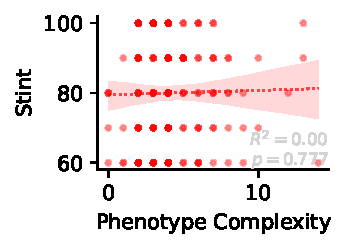
\includegraphics[width=0.295\linewidth,trim={0 1.2cm 0 0},clip]{binder-2025-12-10-complexty-fitness-correlation.ipynb/binder/teeplots/2025-12-10-complexty-fitness-correlation/agg=False+viz=lmplot+when=late+x=phenotype-complexity+y=stint+ext=.pdf}
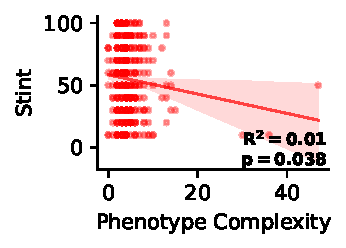
\includegraphics[width=0.295\linewidth,trim={0 1.2cm 0 0},clip]{binder-2025-12-10-complexty-fitness-correlation.ipynb/binder/teeplots/2025-12-10-complexty-fitness-correlation/agg=False+viz=lmplot+when=all+x=phenotype-complexity+y=stint+ext=.pdf}

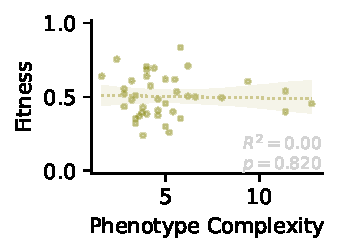
\includegraphics[width=0.39\linewidth,trim={0 1.2cm 0 0},clip]{binder-2025-12-10-complexty-fitness-correlation.ipynb/binder/teeplots/2025-12-10-complexty-fitness-correlation/agg=True+viz=lmplot+when=early+x=phenotype-complexity+y=focal-prevalence+ext=.pdf}
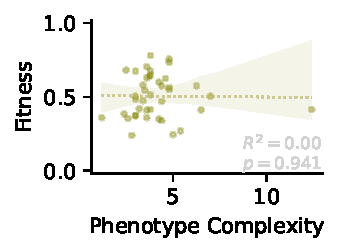
\includegraphics[width=0.295\linewidth,trim={1.45cm 1.2cm 0 0},clip]{binder-2025-12-10-complexty-fitness-correlation.ipynb/binder/teeplots/2025-12-10-complexty-fitness-correlation/agg=True+viz=lmplot+when=late+x=phenotype-complexity+y=focal-prevalence+ext=.pdf}
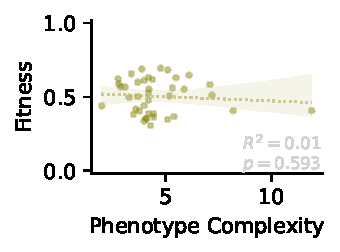
\includegraphics[width=0.295\linewidth,trim={1.45cm 1.2cm 0 0},clip]{binder-2025-12-10-complexty-fitness-correlation.ipynb/binder/teeplots/2025-12-10-complexty-fitness-correlation/agg=True+viz=lmplot+when=all+x=phenotype-complexity+y=focal-prevalence+ext=.pdf}

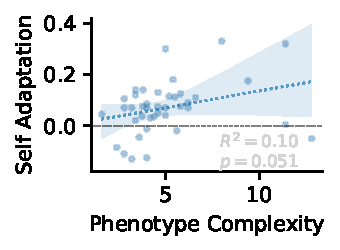
\includegraphics[align=t,width=0.39\linewidth,trim={0 0.7cm 0 0},clip]{binder-2025-12-10-complexty-fitness-correlation.ipynb/binder/teeplots/2025-12-10-complexty-fitness-correlation/viz=lmplot+when=early+x=phenotype-complexity+y=focal-prevalence-difference+ext=.pdf}
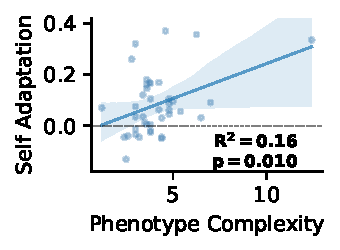
\includegraphics[align=t,width=0.295\linewidth,trim={1.45cm 0.7cm 0 0},clip]{binder-2025-12-10-complexty-fitness-correlation.ipynb/binder/teeplots/2025-12-10-complexty-fitness-correlation/viz=lmplot+when=late+x=phenotype-complexity+y=focal-prevalence-difference+ext=.pdf}
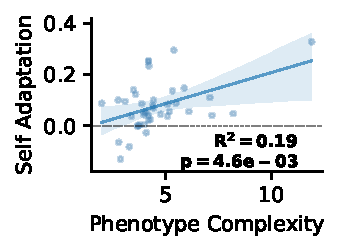
\includegraphics[align=t,width=0.295\linewidth,trim={1.45cm 0.7cm 0 0},clip]{binder-2025-12-10-complexty-fitness-correlation.ipynb/binder/teeplots/2025-12-10-complexty-fitness-correlation/viz=lmplot+when=all+x=phenotype-complexity+y=focal-prevalence-difference+ext=.pdf}
\vspace{-0.75em}
\caption{\footnotesize
phenotype complexity
}
\label{fig:fit-advantage-correlations-supp:phenotype}
\end{subfigure}\\

\begin{subfigure}{0.5\linewidth}
\begin{minipage}{0.1\linewidth}
~
\end{minipage}%
\begin{minipage}{0.3\linewidth}
\centering
\textit{Early}
\end{minipage}%
\begin{minipage}{0.3\linewidth}
\centering
\textit{Late}
\end{minipage}%
\begin{minipage}{0.3\linewidth}
\centering
\textit{All}
\end{minipage}
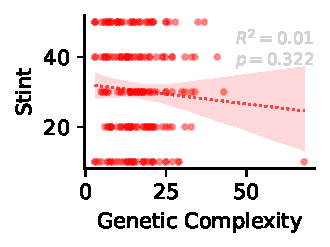
\includegraphics[width=0.39\linewidth,trim={0 1.2cm 0 0},clip]{binder-2025-12-10-complexty-fitness-correlation.ipynb/binder/teeplots/2025-12-10-complexty-fitness-correlation/agg=False+viz=lmplot+when=early+x=genetic-complexity+y=stint+ext=.pdf}
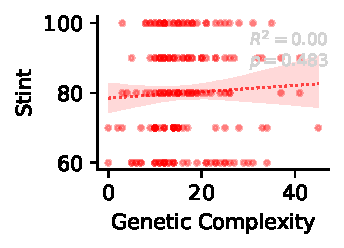
\includegraphics[width=0.295\linewidth,trim={0 1.2cm 0 0},clip]{binder-2025-12-10-complexty-fitness-correlation.ipynb/binder/teeplots/2025-12-10-complexty-fitness-correlation/agg=False+viz=lmplot+when=late+x=genetic-complexity+y=stint+ext=.pdf}
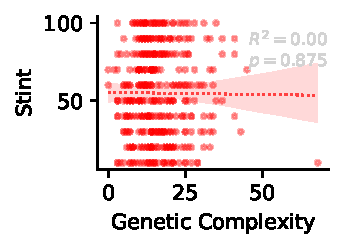
\includegraphics[width=0.295\linewidth,trim={0 1.2cm 0 0},clip]{binder-2025-12-10-complexty-fitness-correlation.ipynb/binder/teeplots/2025-12-10-complexty-fitness-correlation/agg=False+viz=lmplot+when=all+x=genetic-complexity+y=stint+ext=.pdf}

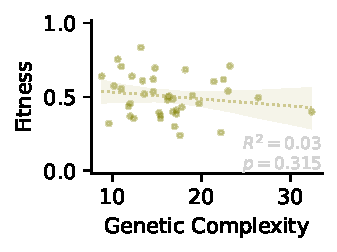
\includegraphics[width=0.39\linewidth,trim={0 1.2cm 0 0},clip]{binder-2025-12-10-complexty-fitness-correlation.ipynb/binder/teeplots/2025-12-10-complexty-fitness-correlation/agg=True+viz=lmplot+when=early+x=genetic-complexity+y=focal-prevalence+ext=.pdf}
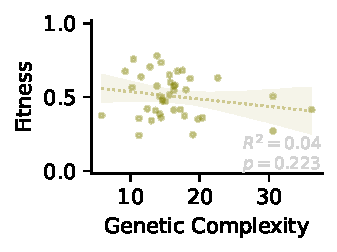
\includegraphics[width=0.295\linewidth,trim={1.45cm 1.2cm 0 0},clip]{binder-2025-12-10-complexty-fitness-correlation.ipynb/binder/teeplots/2025-12-10-complexty-fitness-correlation/agg=True+viz=lmplot+when=late+x=genetic-complexity+y=focal-prevalence+ext=.pdf}
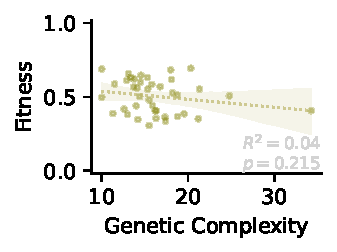
\includegraphics[width=0.295\linewidth,trim={1.45cm 1.2cm 0 0},clip]{binder-2025-12-10-complexty-fitness-correlation.ipynb/binder/teeplots/2025-12-10-complexty-fitness-correlation/agg=True+viz=lmplot+when=all+x=genetic-complexity+y=focal-prevalence+ext=.pdf}

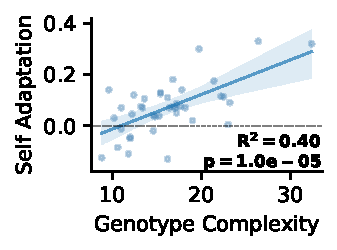
\includegraphics[align=t,width=0.39\linewidth,trim={0 0.7cm 0 0},clip]{binder-2025-12-10-complexty-fitness-correlation.ipynb/binder/teeplots/2025-12-10-complexty-fitness-correlation/viz=lmplot+when=early+x=genotype-complexity+y=focal-prevalence-difference+ext=.pdf}
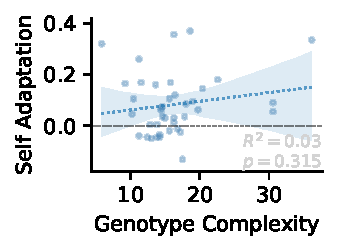
\includegraphics[align=t,width=0.295\linewidth,trim={1.45cm 0.7cm 0 0},clip]{binder-2025-12-10-complexty-fitness-correlation.ipynb/binder/teeplots/2025-12-10-complexty-fitness-correlation/viz=lmplot+when=late+x=genotype-complexity+y=focal-prevalence-difference+ext=.pdf}
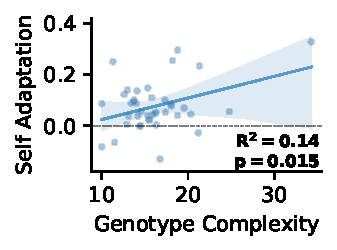
\includegraphics[align=t,width=0.295\linewidth,trim={1.45cm 0.7cm 0 0},clip]{binder-2025-12-10-complexty-fitness-correlation.ipynb/binder/teeplots/2025-12-10-complexty-fitness-correlation/viz=lmplot+when=all+x=genotype-complexity+y=focal-prevalence-difference+ext=.pdf}
\vspace{-0.75em}
\caption{\footnotesize
genotype complexity
}
\label{fig:fit-advantage-correlations-supp:genotype}
\end{subfigure}%
\begin{subfigure}{0.5\linewidth}
\begin{minipage}{0.1\linewidth}
~
\end{minipage}%
\begin{minipage}{0.3\linewidth}
\centering
\textit{Early}
\end{minipage}%
\begin{minipage}{0.3\linewidth}
\centering
\textit{Late}
\end{minipage}%
\begin{minipage}{0.3\linewidth}
\centering
\textit{All}
\end{minipage}

\includegraphics[width=0.33\linewidth,trim={0 0 0 0},clip]{binder-2026-02-04-cryptic-complexity.ipynb/binder/teeplots/2026-02-04-cryptic-complexity/agg=False+kind=None+viz=lmplot+when=early+x=stint+y=genotype-complexity+ext=.pdf}%
\includegraphics[width=0.33\linewidth,trim={0 0 0 0},clip]{binder-2026-02-04-cryptic-complexity.ipynb/binder/teeplots/2026-02-04-cryptic-complexity/agg=False+kind=None+viz=lmplot+when=late+x=stint+y=genotype-complexity+ext=.pdf}%
\includegraphics[width=0.33\linewidth,trim={0 0 0 0},clip]{binder-2026-02-04-cryptic-complexity.ipynb/binder/teeplots/2026-02-04-cryptic-complexity/agg=False+kind=None+viz=lmplot+when=all+x=stint+y=genotype-complexity+ext=.pdf}

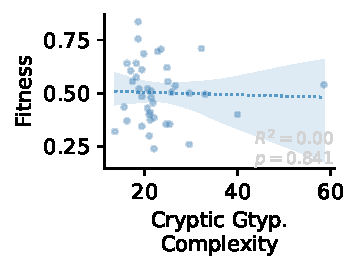
\includegraphics[width=0.33\linewidth,trim={0 0 0 0},clip]{binder-2026-02-04-cryptic-complexity.ipynb/binder/teeplots/2026-02-04-cryptic-complexity/kind=none+viz=lmplot+when=early+x=genotype-complexity+y=focal-prevalence+ext=.pdf}%
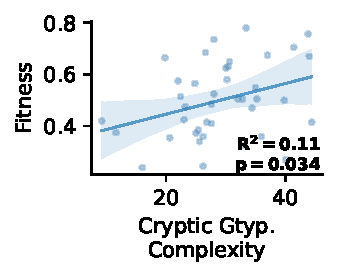
\includegraphics[width=0.33\linewidth,trim={0 0 0 0},clip]{binder-2026-02-04-cryptic-complexity.ipynb/binder/teeplots/2026-02-04-cryptic-complexity/kind=none+viz=lmplot+when=late+x=genotype-complexity+y=focal-prevalence+ext=.pdf}%
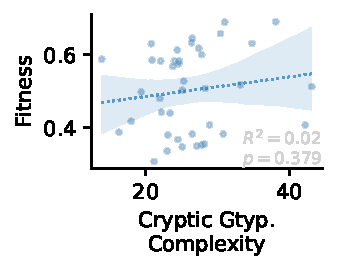
\includegraphics[width=0.33\linewidth,trim={0 0 0 0},clip]{binder-2026-02-04-cryptic-complexity.ipynb/binder/teeplots/2026-02-04-cryptic-complexity/kind=none+viz=lmplot+when=all+x=genotype-complexity+y=focal-prevalence+ext=.pdf}

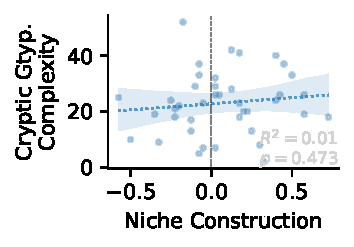
\includegraphics[width=0.33\linewidth,trim={0 0 0 0},clip]{binder-2026-02-04-cryptic-complexity.ipynb/binder/teeplots/2026-02-04-cryptic-complexity/kind=None+viz=lmplot+when=early+x=focal-prevalence-difference+y=genotype-complexity+ext=.pdf}%
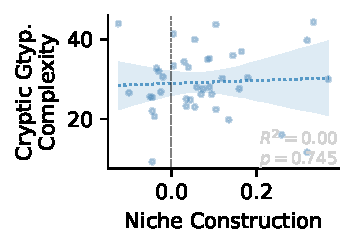
\includegraphics[width=0.33\linewidth,trim={0 0 0 0},clip]{binder-2026-02-04-cryptic-complexity.ipynb/binder/teeplots/2026-02-04-cryptic-complexity/kind=None+viz=lmplot+when=late+x=focal-prevalence-difference+y=genotype-complexity+ext=.pdf}%
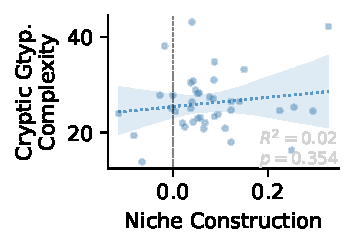
\includegraphics[width=0.33\linewidth,trim={0 0 0 0},clip]{binder-2026-02-04-cryptic-complexity.ipynb/binder/teeplots/2026-02-04-cryptic-complexity/kind=None+viz=lmplot+when=all+x=focal-prevalence-difference+y=genotype-complexity+ext=.pdf}

\vspace{-0.75em}
\caption{\footnotesize
deep (cryptic) genotype complexity
}
\label{fig:fit-advantage-correlations-supp:deep-genotype-cryptic}
\end{subfigure}

\caption{
\textbf{Co-occurrence of drift (time), niche construction (self adaptation), and fitness with complexity across replicates.}
\footnotesize
Pearson correlation and two-tail Wald tests reported.
}
\label{fig:fit-advantage-correlations-supp}

\end{figure*}
